\tocless\subsection{Proof}

We are ready to tackle the general proof which allows us to show that any full program reduction that happens under \tpl\ semantics can be replicated by the \textsc{Atom} one. This relation will be verified with regards to the final storage achieved by the reductions under the two different semantics. The first level of proof is an induction on the syntactic structure of programs.

The single transaction case $\ptdef{\mathds{C}}$ follows from the single step equivalence of the two operational semantics when reducing sequential commands (i.e. the transaction's body $\mathds{C}$). In the case of a loop $\mathds{P}^*$ and of nondeterministic choice $\mathds{P}_1 + \mathds{P}_2$ we get the needed result from the inductive hypothesys on $\mathds{P}$ and $\mathds{P}_1, \mathds{P}_2$ respectively. The sequential composition of programs is dealt with using a series of auxiliary lemmata together with the inductive hypothesis on $\mathds{P}_1, \mathds{P}_2$. Parallel composition is, as expected, the most challenging case, and its proof requires a particular multi-step strategy summarized at an intuitive level below.
\begin{enumerate}
	\item Retrieve a full trace $\tau$ from the terminating reduction of $\mathds{P}_1 \| \mathds{P}_2$.
	\[\footnotesize
		\begin{tikzpicture}[->, semithick]
			\tikzset{
			    tsys/.style= {rectangle, draw=black, color=black, minimum height=0.65cm},
			    t1/.style= {rectangle, draw=blue, color=blue, minimum height=0.65cm},
			    t2/.style= {rectangle, draw=magenta, color=magenta, minimum height=0.65cm},
			    t3/.style= {rectangle, draw=orange, color=orange, minimum height=0.65cm},
			}
			
			\node[tsys] (s1) at (0, 0) {$\actprog$};
			\node[t1] (s2) at (1.5, 0) {$\actlock{1}{5}{\textsc{s}}$};
			\node[t2] (s3) at (3.65, 0) {$\actlock{2}{7}{\textsc{x}}$};
			\node[t2] (s4) at (5.85, 0) {$\actwrite{2}{7}{1}$};
			\node[t2] (s5) at (8.05, 0) {$\actunlock{2}{7}$};
			\node[t3] (s6) at (10.2, 0) {$\actlock{3}{7}{\textsc{x}}$};
			\node[t3] (s7) at (12.35, 0) {$\actread{3}{7}{1}$};
			\node[t1] (s8) at (0.625, -1) {$\actlock{1}{6}{\textsc{s}}$};
			\node[t3] (s9) at (2.8, -1) {$\actunlock{3}{7}$};
			\node[t1] (s10) at (4.95, -1) {$\actread{1}{6}{0}$};
			\node[t2] (s11) at (6.6, -1) {$\actid{2}$};
			\node[t1] (s12) at (8.25, -1) {$\actunlock{1}{5}$};
			\node[t1] (s12) at (10.4, -1) {$\actunlock{1}{6}$};
		\end{tikzpicture}
	\]
	
	\item Clean $\tau$ from any spurious locks that appear inside of it in order to obtain $\tau'$.
	\[\footnotesize
		\begin{tikzpicture}[->, semithick]
			\tikzset{
			    tsys/.style= {rectangle, draw=black, color=black, minimum height=0.65cm, opacity=0.5},
			    t1/.style= {rectangle, draw=blue, color=blue, minimum height=0.65cm, opacity=0.5},
			    t2/.style= {rectangle, draw=magenta, color=magenta, minimum height=0.65cm, opacity=0.5},
			    t3/.style= {rectangle, draw=orange, color=orange, minimum height=0.65cm, opacity=0.5},
			}
			
			\node[tsys] (s1) at (0, 0) {$\actprog$};
			\node[t1, opacity=1, cross out] (s2) at (1.5, 0) {$\actlock{1}{5}{\textsc{s}}$};
			\node[t2] (s3) at (3.65, 0) {$\actlock{2}{7}{\textsc{x}}$};
			\node[t2] (s4) at (5.85, 0) {$\actwrite{2}{7}{1}$};
			\node[t2] (s5) at (8.05, 0) {$\actunlock{2}{7}$};
			\node[t3] (s6) at (10.2, 0) {$\actlock{3}{7}{\textsc{x}}$};
			\node[t3] (s7) at (12.35, 0) {$\actread{3}{7}{1}$};
			\node[t1] (s8) at (0.625, -1) {$\actlock{1}{6}{\textsc{s}}$};
			\node[t3] (s9) at (2.8, -1) {$\actunlock{3}{7}$};
			\node[t1] (s10) at (4.95, -1) {$\actread{1}{6}{0}$};
			\node[t2] (s11) at (6.6, -1) {$\actid{2}$};
			\node[t1, opacity=1, cross out] (s12) at (8.25, -1) {$\actunlock{1}{5}$};
			\node[t1] (s12) at (10.4, -1) {$\actunlock{1}{6}$};
		\end{tikzpicture}
	\]
	
	\item Convert any redundant exclusive lock in $\tau'$ into a shared one and compute $\tau_{c}$.
	\[\footnotesize
		\begin{tikzpicture}[->, semithick]
			\tikzset{
			    tsys/.style= {rectangle, draw=black, color=black, minimum height=0.65cm, opacity=0.5},
			    t1/.style= {rectangle, draw=blue, color=blue, minimum height=0.65cm, opacity=0.5},
			    t2/.style= {rectangle, draw=magenta, color=magenta, minimum height=0.65cm, opacity=0.5},
			    t3/.style= {rectangle, draw=orange, color=orange, minimum height=0.65cm, opacity=0.5},
			}
			
			\node[tsys] (s1) at (0, 0) {$\actprog$};
			\node[t2, opacity=0.5] (s3) at (3.65, 0) {$\actlock{2}{7}{\textsc{x}}$};
			\node[t2] (s4) at (5.85, 0) {$\actwrite{2}{7}{1}$};
			\node[t2] (s5) at (8.05, 0) {$\actunlock{2}{7}$};
			\node[t3, opacity=1, fill=orange, text=white] (s6) at (10.2, 0) {$\actlock{3}{7}{\textsc{s}}$};
			\node[t3] (s7) at (12.35, 0) {$\actread{3}{7}{1}$};
			\node[t1] (s8) at (0.625, -1) {$\actlock{1}{6}{\textsc{s}}$};
			\node[t3] (s9) at (2.8, -1) {$\actunlock{3}{7}$};
			\node[t1] (s10) at (4.95, -1) {$\actread{1}{6}{0}$};
			\node[t2] (s11) at (6.6, -1) {$\actid{2}$};
			\node[t1] (s12) at (10.4, -1) {$\actunlock{1}{6}$};
		\end{tikzpicture}
	\]
	
	\item Build a serialization graph out of $\tau_{c}$.
	\[
		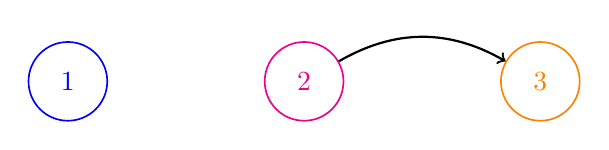
\begin{tikzpicture}[->, semithick]
			\tikzset{
			    tnode/.style= {circle, draw=blue, color=blue, minimum width=1cm},
			    pnew/.style= {below, black!5!black, thick},
			}
			
			\node[tnode] (s1) at (0, 0) {$1$};
			\node[tnode, color=magenta] (s2) at (3, 0) {$2$};
			\node[tnode, color=orange] (s3) at (6, 0) {$3$};
			
			\draw
			(s2) edge[pnew, bend left] (s3);
		\end{tikzpicture}
	\]
	
	\item Extend the serialization graph to the strict total order $\sqsubset$ and find its minimal element $\iota$.
	\[
		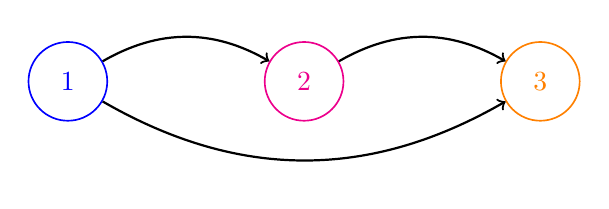
\begin{tikzpicture}[->, semithick]
			\tikzset{
			    tnode/.style= {circle, draw=blue, color=blue, minimum width=1cm},
			    pnew/.style= {below, black!5!black, thick},
			}
			
			\node[tnode] (s1) at (0, 0) {$1$};
			\node[tnode, color=magenta] (s2) at (3, 0) {$2$};
			\node[tnode, color=orange] (s3) at (6, 0) {$3$};
			
			\draw
			(s1) edge[pnew, bend left] (s2)
			(s1) edge[pnew, bend right] (s3)
			(s2) edge[pnew, bend left] (s3);
		\end{tikzpicture}
	\]
	
	\item Swap all of $\iota$'s operations to the left of the trace until no swap is possible anymore. The final trace will be $\tau_{seq}$.
	\[\footnotesize
		\begin{tikzpicture}[->, semithick]
			\tikzset{
			    tsys/.style= {rectangle, draw=black, color=black, minimum height=0.65cm},
			    t1/.style= {rectangle, draw=blue, color=blue, minimum height=0.65cm},
			    t2/.style= {rectangle, draw=magenta, color=magenta, minimum height=0.65cm},
			    t3/.style= {rectangle, draw=orange, color=orange, minimum height=0.65cm},
			}
			
			\node[tsys] (s1) at (0, 0) {$\actprog$};
			\node[t1] (s2) at (1.5, 0) {$\actlock{1}{6}{\textsc{s}}$};
			\node[t1] (s10) at (3.65, 0) {$\actread{1}{6}{0}$};
			\node[t1] (s12) at (5.8, 0) {$\actunlock{1}{6}$};
			\node[t2] (s5) at (7.95, 0) {$\actlock{2}{7}{\textsc{x}}$};
			\node[t2] (s6) at (10.15, 0) {$\actwrite{2}{7}{1}$};
			\node[t2] (s7) at (12.35, 0) {$\actunlock{2}{7}$};
			\node[t3] (s8) at (0.64, -1) {$\actlock{3}{7}{\textsc{x}}$};
			\node[t3] (s7) at (2.8, -1) {$\actread{3}{7}{1}$};
			\node[t3] (s9) at (4.95, -1) {$\actunlock{3}{7}$};
			\node[t2] (s11) at (6.6, -1) {$\actid{2}$};
		\end{tikzpicture}
	\]
	
	\item Show that no operation done by another transaction can appear in $\tau_{seq}$ before one done by $\iota$.
	\[\footnotesize
		\begin{tikzpicture}[semithick]
			\tikzset{
			    tsys/.style= {rectangle, draw=black, color=black, minimum height=0.65cm, opacity=0.5},
			    t1/.style= {rectangle, draw=blue, color=blue, minimum height=0.65cm},
			    t2/.style= {rectangle, draw=magenta, color=magenta, minimum height=0.65cm, opacity=0.5},
			    t3/.style= {rectangle, draw=orange, color=orange, minimum height=0.65cm, opacity=0.5},
			}
			
			\node[tsys] (s1) at (0, 0) {$\actprog$};
			\node[t1] (s2) at (1.5, 0) {$\actlock{1}{6}{\textsc{s}}$};
			\node[t1] (s10) at (3.65, 0) {$\actread{1}{6}{0}$};
			\node[t1] (s12) at (5.8, 0) {$\actunlock{1}{6}$};
			\node[t2] (s5) at (7.95, 0) {$\actlock{2}{7}{\textsc{x}}$};
			\node[t2] (s6) at (10.15, 0) {$\actwrite{2}{7}{1}$};
			\node[t2] (s7) at (12.35, 0) {$\actunlock{2}{7}$};
			\node[t3] (s8) at (0.64, -1) {$\actlock{3}{7}{\textsc{x}}$};
			\node[t3] (s7) at (2.8, -1) {$\actread{3}{7}{1}$};
			\node[t3] (s9) at (4.95, -1) {$\actunlock{3}{7}$};
			\node[t2] (s11) at (6.6, -1) {$\actid{2}$};
			
			\draw[thick] (0.45, 0.15) -- (0.45, 0.5) -- node[midway, above] {1 \checkmark} (6.875, 0.5) -- (6.875, 0.15);
		\end{tikzpicture}
	\]
	
	\item Replicate any system transition labelled with $\actprog$ in the \textsc{Atom} semantics, knowing that the state does not change.
	\[\footnotesize
		\begin{tikzpicture}[semithick]
			\tikzset{
			    tsys/.style= {rectangle, text=white, fill=black, minimum height=0.65cm},
			    t1/.style= {rectangle, draw=blue, color=blue, minimum height=0.65cm, opacity=0.5},
			    t2/.style= {rectangle, draw=magenta, color=magenta, minimum height=0.65cm, opacity=0.5},
			    t3/.style= {rectangle, draw=orange, color=orange, minimum height=0.65cm, opacity=0.5},
			}
			
			\node[tsys] (s1) at (0, 0) {$\actprog$};
			\node[t1] (s2) at (1.5, 0) {$\actlock{1}{6}{\textsc{s}}$};
			\node[t1] (s10) at (3.65, 0) {$\actread{1}{6}{0}$};
			\node[t1] (s12) at (5.8, 0) {$\actunlock{1}{6}$};
			\node[t2] (s5) at (7.95, 0) {$\actlock{2}{7}{\textsc{x}}$};
			\node[t2] (s6) at (10.15, 0) {$\actwrite{2}{7}{1}$};
			\node[t2] (s7) at (12.35, 0) {$\actunlock{2}{7}$};
			\node[t3] (s8) at (0.64, -1) {$\actlock{3}{7}{\textsc{x}}$};
			\node[t3] (s7) at (2.8, -1) {$\actread{3}{7}{1}$};
			\node[t3] (s9) at (4.95, -1) {$\actunlock{3}{7}$};
			\node[t2] (s11) at (6.6, -1) {$\actid{2}$};
			
			\draw[->, thick] (-0.33, 0.6) -- (0.435, 0.6) -- (0.435, 0.3);
		\end{tikzpicture}
	\]
	
	\item Use the semantics equivalence for a single transaction together with the inductive hypothesis to conclude the proof.
	\[\footnotesize
		\begin{tikzpicture}[semithick]
			\tikzset{
			    tsys/.style= {rectangle, text=white, fill=black, minimum height=0.65cm},
			    t1/.style= {rectangle, text=white, fill=blue, minimum height=0.65cm},
			    t2/.style= {rectangle, draw=magenta, color=magenta, minimum height=0.65cm, opacity=0.5},
			    t3/.style= {rectangle, draw=orange, color=orange, minimum height=0.65cm, opacity=0.5},
			}
			
			\node[tsys] (s1) at (0, 0) {$\actprog$};
			\node[t1] (s2) at (1.5, 0) {$\actlock{1}{6}{\textsc{s}}$};
			\node[t1] (s10) at (3.65, 0) {$\actread{1}{6}{0}$};
			\node[t1] (s12) at (5.8, 0) {$\actunlock{1}{6}$};
			\node[t2] (s5) at (7.95, 0) {$\actlock{2}{7}{\textsc{x}}$};
			\node[t2] (s6) at (10.15, 0) {$\actwrite{2}{7}{1}$};
			\node[t2] (s7) at (12.35, 0) {$\actunlock{2}{7}$};
			\node[t3] (s8) at (0.64, -1) {$\actlock{3}{7}{\textsc{x}}$};
			\node[t3] (s7) at (2.8, -1) {$\actread{3}{7}{1}$};
			\node[t3] (s9) at (4.95, -1) {$\actunlock{3}{7}$};
			\node[t2] (s11) at (6.6, -1) {$\actid{2}$};
			
			\draw[->, thick] (-0.33, 0.6) -- (6.865, 0.6) -- (6.865, 0.3);
			\draw[->, dashed] (7.1, 0.6) -- node[near start, above] {I.H.} (11, 0.6);
		\end{tikzpicture}
	\]
\end{enumerate}

\begin{thm}

\label{thm:atom}

\[
	\forall h, h', S, S' \ldotp
	(h, \emptyset, S, \mathds{P}) \rightarrow^* (h', \emptyset, S', \pskip) \implies 
	(h, \mathds{P}) \tred^* (h', \pskip)
\]

{\parindent0pt
\begin{proof}
The proof is done by induction on the structure of programs $\mathsf{Prog}$. \\
\indline
\textit{Base case 1}: $\pskip \in \mathsf{Prog}$

\textit{To show}:
\[
	\forall h, h', S, S' \ldotp
	(h, \emptyset, S, \pskip) \rightarrow^* (h', \emptyset, S', \pskip) \implies 
	(h, \pskip) \tred^* (h', \pskip)
\]

For arbitrary $h, h', S, S'$ we assume that $(h, \emptyset, S, \pskip) \rightarrow^* (h', \emptyset, S', \pskip)$ holds, and given that $\pskip$ has no possible one-step reductions, it must be the case that it is a zero-step reduction. Therefore we have $h = h'$ and $S = S'$. Starting from $(h, \pskip)$ through the $\tred$ relation, we can always reach $(h, \pskip)$ via a zero-step reduction $(h, \pskip) \tred^0 (h, \pskip)$. We can conclude that $(h, \emptyset, S, \pskip) \rightarrow^* (h', \emptyset, S', \pskip) \implies (h, \pskip) \tred^* (h', \pskip)$ where $h = h'$. \\
\indline
\textit{Base case 2}: $\mathds{T} \in \mathsf{Prog}$

\textit{To show}:
\[
	\forall h, h', S, S' \ldotp
	(h, \emptyset, S, \mathds{T}) \rightarrow^* (h', \emptyset, S', \pskip) \implies 
	(h, \mathds{T}) \tred^* (h', \pskip)
\]

We will proceed with the proof by induction on the structure of transactions $\mathsf{Trans}$. Given that the \textsc{Atom} semantics only support user transactions, all that is required to show is:
\begin{gather*}
	\forall h, h', S, S' \ldotp \\
	(h, \emptyset, S, \ptdef{\mathds{C}}) \rightarrow^* (h', \emptyset, S', \pskip) \implies 
	(h, \ptdef{\mathds{C}}) \tred^* (h', \pskip)
\end{gather*}

For arbitrary $h, h', S, S'$ we assume that $(h, \emptyset, S, \ptdef{\mathds{C}}) \rightarrow^* (h', \emptyset, S', \pskip)$ holds. Given the overall reduction from $\ptdef{\mathds{C}}$ to $\pskip$ it must be the case that the following holds.
\begin{gather*}
	(h, \emptyset, S, \ptdef{\mathds{C}})
	\xrightarrow{\actid{\iota}} (h, \emptyset, S[\iota \mapsto (\emptyset, \pgrow)], \ptdef{\mathds{C}}_\iota) \\
	\rightarrow^* (h', \emptyset, S', \ptdef{\pskip}_\iota)
	\xrightarrow{\actprog} (h', \emptyset, S', \pskip)
\end{gather*}
Which implies that $\mathds{C}$ reduces to $\pskip$ through the repeated use of the \textsc{Exec} rule. From the transitive closure of the $\rightarrow$ relation and Lemma \ref{lem:catom} we obtain the result that $(h, \ptdef{\mathds{C}}) \tred^* (h', \pskip)$. \\
\indline
\textit{Inductive case 1}: $\mathds{P}_1 + \mathds{P}_2 \in \mathsf{Prog}$

\textit{To show}:
\[
	\forall h, h', S, S' \ldotp
	(h, \emptyset, S, \mathds{P}_1 + \mathds{P}_2) \rightarrow^* (h', \emptyset, S', \pskip) \implies 
	(h, \mathds{P}_1 + \mathds{P}_2 ) \tred^* (h', \pskip)
\]

\textit{Inductive hypothesis}:
\begin{gather*}
	\forall h, h', S, S' \ldotp
	(h, \emptyset, S, \mathds{P}_1) \rightarrow^* (h', \emptyset, S', \pskip) \implies 
	(h, \mathds{P}_1) \tred^* (h', \pskip)
	\\ \land \\
	\forall h, h', S, S' \ldotp
	(h, \emptyset, S, \mathds{P}_2) \rightarrow^* (h', \emptyset, S', \pskip) \implies 
	(h, \mathds{P}_2) \tred^* (h', \pskip)
\end{gather*}

For arbitrary $h, h', S, S'$ we assume that $(h, \emptyset, S, \mathds{P}_1 + \mathds{P}_2) \rightarrow^* (h', \emptyset, S', \pskip)$ holds. Now we are presented with two cases:
\begin{enumerate}
	\item We can reduce $(h, \emptyset, S, \mathds{P}_1 + \mathds{P}_2) \xrightarrow{\actprog} (h, \emptyset, S, \mathds{P}_1)$ with one step through the \textsc{ChoiceL} rule, which we can always apply since it has an empty premiss. We can also always reduce $(h, \mathds{P}_1 + \mathds{P}_2) \tred (h, \mathds{P}_1)$ through the rule \textsc{AtChoiceL} given it has an empty premiss. By inductive hypothesis on $\mathds{P}_1$ we obtain that $(h, \emptyset, S, \mathds{P}_1) \rightarrow^* (h', \emptyset, S', \pskip) \implies (h, \mathds{P}_1) \tred^* (h', \pskip)$. Therefore we can conclude that:
	\[
		(h, \emptyset, S, \mathds{P}_1 + \mathds{P}_2) \rightarrow^* (h', \emptyset, S', \pskip) \implies  (h, \mathds{P}_1 + \mathds{P}_2) \tred^* (h', \pskip)
	\]
	
	\item We can reduce $(h, \emptyset, S, \mathds{P}_1 + \mathds{P}_2) \xrightarrow{\actprog} (h, \emptyset, S, \mathds{P}_2)$ with one step through the \textsc{ChoiceR} rule, which we can always apply since it has an empty premiss. We can also always reduce $(h, \mathds{P}_1 + \mathds{P}_2) \tred (h, \mathds{P}_2)$ through the rule \textsc{AtChoiceR} given it has an empty premiss. By inductive hypothesis on $\mathds{P}_2$ we obtain that $(h, \emptyset, S, \mathds{P}_2) \rightarrow^* (h', \emptyset, S', \pskip) \implies (h, \mathds{P}_2) \tred^* (h', \pskip)$. Therefore we can conclude that:
	\[
		(h, \emptyset, S, \mathds{P}_1 + \mathds{P}_2) \rightarrow^* (h', \emptyset, S', \pskip) \implies  (h, \mathds{P}_1 + \mathds{P}_2) \tred^* (h', \pskip)
	\]
\end{enumerate}
\indline
\textit{Inductive case 2}: $\mathds{P}_1 ; \mathds{P}_2 \in \mathsf{Prog}$

\textit{To show}:
\[
	\forall h, h', S, S' \ldotp
	(h, \emptyset, S, \mathds{P}_1 ; \mathds{P}_2) \rightarrow^* (h', \emptyset, S', \pskip) \implies 
	(h, \mathds{P}_1 ; \mathds{P}_2 ) \tred^* (h', \pskip)
\]

\textit{Inductive hypothesis}:
\begin{gather*}
	\forall h, h', S, S' \ldotp
	(h, \emptyset, S, \mathds{P}_1) \rightarrow^* (h', \emptyset, S', \pskip) \implies 
	(h, \mathds{P}_1) \tred^* (h', \pskip)
	\\ \land \\
	\forall h, h', S, S' \ldotp
	(h, \emptyset, S, \mathds{P}_2) \rightarrow^* (h', \emptyset, S', \pskip) \implies 
	(h, \mathds{P}_2) \tred^* (h', \pskip)
\end{gather*}

For arbitrary $h, h', S, S'$ we assume that $(h, \emptyset, S, \mathds{P}_1 ; \mathds{P}_2) \rightarrow^* (h', \emptyset, S', \pskip)$ holds. Given the overall reduction from $\mathds{P}_1 ; \mathds{P}_2$ to $\pskip$ we must have a chain of reductions of the following shape, for some $h'', S'', \Phi''$ and where $\Phi'' = \emptyset$ by Lemma \ref{ref:phiemp}.
\[
	\underbrace{(h, \emptyset, S, \mathds{P}_1 ; \mathds{P}_2) \rightarrow^* (h'', \Phi'', S'', \pskip; \mathds{P}_2)}_{(\textsc{i})}
	\xrightarrow{\actprog} (h'', \emptyset, S'', \mathds{P}_2) \rightarrow^* (h', \emptyset, S', \pskip)
\]
\begin{enumerate}
	\item \label{seq:1} By (\textsc{i}) and Lemma \ref{ref:2seq} we get that $(h, \emptyset, S, \mathds{P}_1) \rightarrow^* (h'', \emptyset, S'', \pskip)$ holds.
	
	\item \label{seq:2} By \ref{seq:1}. and the inductive hypothesis on $\mathds{P}_1$ we obtain that $(h, \mathds{P}_1) \tred^* (h'', \pskip)$.
	
	\item By \ref{seq:2}. and Lemma \ref{ref:aseq} we get that $(h, \mathds{P}_1 ; \mathds{P}_2) \tred^* (h'', \pskip ; \mathds{P}_2)$.
\end{enumerate}

At this point we can apply the \textsc{PSeqSkip} rule to reduce $(h'', \emptyset, S'', \pskip ; \mathds{P}_2) \xrightarrow{\actprog} (h'', \emptyset, S'', \mathds{P}_2)$ and rule \textsc{AtPSeqSkip} to reduce $(h'', \pskip ; \mathds{P}_2) \tred^* (h'', \mathds{P}_2)$. By inductive hypothesis on $\mathds{P}_2$ we can conclude that $(h, \emptyset, S, \mathds{P}_1 ; \mathds{P}_2) \rightarrow^* (h', \emptyset, S', \pskip) \implies (h, \mathds{P}_1 ; \mathds{P}_2) \tred^* (h', \pskip)$. \\
\indline
\textit{Inductive case 3}: $\mathds{P}^* \in \mathsf{Prog}$

\textit{To show}:
\[
	\forall h, h', S, S' \ldotp
	(h, \emptyset, S, \mathds{P}^*) \rightarrow^* (h', \emptyset, S', \pskip) \implies 
	(h, \mathds{P}^* ) \tred^* (h', \pskip)
\]

\textit{Inductive hypothesis}:
\[
	\forall h, h', S, S' \ldotp
	(h, \emptyset, S, \mathds{P}) \rightarrow^* (h', \emptyset, S', \pskip) \implies 
	(h, \mathds{P}) \tred^* (h', \pskip)
\]

We prove this case by mathematical induction on $n$, the number of $\rightarrow^*$ reduction steps. \\

\textit{Base case 3.1}: $n = 2$

\textit{To show}:
\[
	\forall h, h', S, S', \mathds{P} \ldotp
	(h, \emptyset, S, \mathds{P}^*) \rightarrow^{2} (h', \emptyset, S', \pskip) \implies 
	(h, \mathds{P}^*) \tred^* (h', \pskip)
\]

For arbitrary $h, h', S, S', \mathds{P}$ we assume that $(h, \emptyset, S, \mathds{P}^*) \rightarrow^{2} (h', \emptyset, S', \pskip)$ holds. The only possible reduction that is able to bring $\mathds{P}^*$ to $\pskip$ in exactly $2$ steps is the following:
\[
	(h, \emptyset, S, \mathds{P}^*) \xrightarrow{\actprog} (h, \emptyset, S, \pskip + (\mathds{P} ; \mathds{P}^*)) \xrightarrow{\actprog} (h, \emptyset, S, \pskip)
\]
where the storage $h$ is left unchanged. This result follows from the application of semantic rules \textsc{Loop} and \textsc{ChoiceL}. It follows that we can replicate the same reduction in the \textsc{Atom} semantics using rules \textsc{AtLoop} and \textsc{AtChoiceL} that will bring us to a final state where the storage component is not changed.
\[
	(h, \mathds{P}^*) \tred (h, \pskip + (\mathds{P} ; \mathds{P}^*)) \tred (h, \pskip)
\]
\\
\textit{Inductive case 3.2}: $n > 2$

\textit{Inductive hypothesis}:
\begin{gather*}
	\forall\ 2 \leq m < n, h, h', S, S', \mathds{P} \ldotp \\
	(h, \emptyset, S, \mathds{P}^*) \rightarrow^{m} (h', \emptyset, S', \pskip) \implies 
	(h, \mathds{P}^* ) \tred^* (h', \pskip)
\end{gather*}

\textit{To show}:
\[
	\forall h, h', S, S', \mathds{P} \ldotp
	(h, \emptyset, S, \mathds{P}^*) \rightarrow^{n + 1} (h', \emptyset, S', \pskip) \implies 
	(h, \mathds{P}^* ) \tred^* (h', \pskip)
\]

For arbitrary $h, h', S, S', \mathds{P}$ we assume that $(h, \emptyset, S, \mathds{P}^*) \rightarrow^{n+1} (h', \emptyset, S', \pskip)$. From here we can always apply the \textsc{Loop} rule , as it does not have any requirements on the state, in order to get:
\begin{gather}
	\label{loop:2}
	(h, \emptyset, S, \mathds{P}^*) \xrightarrow{\actprog} (h, \emptyset, S, \pskip + (\mathds{P} ; \mathds{P}^*)) \rightarrow^* (h', \emptyset, S', \pskip)
\end{gather}
From (\ref{loop:2}) there are two possible cases to consider:
\begin{enumerate}
	\item We utilize rule \textsc{ChoiceL} in order to reduce $(h, \emptyset, S, \pskip + (\mathds{P} ; \mathds{P}^*)) \xrightarrow{\actprog} (h, \emptyset, S, \pskip)$, which we can always do. It is now possible to replicate the same reduction in the \textsc{Atom} semantics by applying rule \textsc{AtChoiceL}, which reduces:
	\[
		(h, \pskip + (\mathds{P} ; \mathds{P}^*)) \tred (h, \pskip)
	\]
	In this scenario we directly obtain the final result.
	
	\item We reduce $(h, \emptyset, S, \pskip + (\mathds{P} ; \mathds{P}^*)) \xrightarrow{\actprog} (h, \emptyset, S, \mathds{P} ; \mathds{P}^*)$ through the \textsc{ChoiceR} rule which we can always do, together with \textsc{AtChoiceR} that reduces in the following way:
	\[
		(h, \pskip + (\mathds{P} ; \mathds{P}^*)) \tred (h, \mathds{P} ; \mathds{P}^*)
	\]
	From Lemma \ref{ref:2seq}, Lemma \ref{ref:aseq} and the top-level inductive hypothesis on $\mathds{P}$ we get that:
	\begin{gather}
		\label{loop4}
		(h, \emptyset, S, \mathds{P} ; \mathds{P}^*) \rightarrow^* (h'', \emptyset, S'', \pskip ; \mathds{P}^*) \implies (h, \mathds{P} ; \mathds{P}^*) \tred^* (h'', \pskip ; \mathds{P}^*)
	\end{gather}
	It is now possible to further reduce the states in (\ref{loop4}):
	\[
		\begin{array}{r l}
			(h'', \emptyset, S'', \pskip ; \mathds{P}^*) \xrightarrow{\actprog} (h'', \emptyset, S'', \mathds{P}^*)
			&
			\text{via \textsc{PSeqSkip}}
			\\[0.5em]
			(h'', \pskip ; \mathds{P}^*) \tred (h'', \mathds{P}^*)
			&
			\text{via \textsc{AtPSeqSkip}}
		\end{array}
	\]
	We have now completed a number of $\rightarrow$ reduction steps greater than $1$ meaning that we can use the \textit{inductive hypothesis 3.2} to obtain the required result.
\end{enumerate}
\indline
\textit{Inductive case 4}: $\mathds{P}_1 \| \mathds{P}_2 \in \mathsf{Prog}$

\textit{To show}:
\[
	\forall h, h', S, S' \ldotp
	(h, \emptyset, S, \mathds{P}_1 \| \mathds{P}_2) \rightarrow^* (h', \emptyset, S', \pskip) \implies 
	(h, \mathds{P}_1 \| \mathds{P}_2 ) \tred^* (h', \pskip)
\]

We will prove the parallel composition case by mathematical induction on the number of reduction steps $n$.

\textit{Base case}: $n = 0$

\textit{To show}:
\begin{gather*}
	\forall h, h', S, S', \mathds{P}_1, \mathds{P}_2 \ldotp \\
	(h, \emptyset, S, \mathds{P}_1 \| \mathds{P}_2) \rightarrow^0 (h', \emptyset, S', \pskip)
	\implies
	(h, \mathds{P}_1 \| \mathds{P}_2) \tred^* (h', \pskip)
\end{gather*}

For arbitrary $h, h', S, S', \mathds{P}_1, \mathds{P}_2$ we assume that $(h, \emptyset, S, \mathds{P}_1 \| \mathds{P}_2) \rightarrow^0 (h', \emptyset, S', \pskip)$ holds. Since a zero-step reduction happened, it must be the case that $\mathds{P}_1 = \mathds{P}_2 = \pskip$, $h' = h$ and $\pskip \| \pskip$ reduced to $\pskip$ through the \textsc{ParEnd} rule. Now, we immediately obtain that $(h, \pskip \| \pskip) \tred (h, \pskip)$ from rule \textsc{AtParEnd}. \\

\textit{Inductive case 4.1}: $n > 0$

\textit{Inductive hypothesis}:
\begin{gather*}
	\forall m \leq n, h, h', S, S', \mathds{P}_1, \mathds{P}_2 \ldotp \\
	(h, \emptyset, S, \mathds{P}_1 \| \mathds{P}_2) \rightarrow^m (h', \emptyset, S', \pskip)
	\implies
	(h, \mathds{P}_1 \| \mathds{P}_2) \tred^* (h', \pskip)
\end{gather*}

\textit{To show}:
\begin{gather*}
	\forall h, h', \Phi, S, S', \mathds{P}_1, \mathds{P}_2 \ldotp \\
	(h, \emptyset, S, \mathds{P}_1 \| \mathds{P}_2) \rightarrow^{n+1} (h', \emptyset, S', \pskip)
	\implies
	(h, \mathds{P}_1 \| \mathds{P}_2) \tred^* (h', \pskip)
\end{gather*}
For arbitrary $h, h', S, S', \mathds{P}_1, \mathds{P}_2$ we assume that $(h, \emptyset, S, \mathds{P}_1 \| \mathds{P}_2) \rightarrow^{n+1} (h', \emptyset, S', \pskip)$ holds. As a consequence, from the definition of $\mathsf{trace}$ and $\mathsf{tgen}$ we can state there is a trace $\tau \in [\mathsf{Act} \times \mathds{N}]$ of length $n + 1$ such that:
\begin{gather}
	\label{thm:atom1}
	\tau = \pred{trace}{h, \emptyset, S, \mathds{P}_1 \| \mathds{P}_2} \land \pred{tgen}{\tau, h, h', \emptyset, S, \mathds{P}_1 \| \mathds{P}_2}
\end{gather}
By repeatedly applying Lemma \ref{lem:lockAbsent} until convergence, we obtain a trace $\tau_c \in [\mathsf{Act} \times \mathds{N}]$ such that $\tau_c$ does not contain spurious lock and unlock operations, i.e. $\pred{clean}{\tau_c}$ holds, and for which the following is true, from (\ref{thm:atom1}).
\begin{gather}
	\label{thm:atom2} \pred{tgen}{\tau_c, h, h', \emptyset, S, \mathds{P}_1 \| \mathds{P}_2}
\end{gather}

From Theorem \ref{thm:totOrder} we are always able to build the strict total order $\sqsubset$ on the set of transactions $N$ that appear in $\tau_c$, for which $(N, E) = \pred{SG}{\tau}$.

From the definition of strict total order, we know we can find the minimal (or first) element $\iota$ of $\sqsubset$ such that:
\begin{gather}
	\label{thm:atom3} \forall j \in N \ldotp \iota \neq j \implies \iota \sqsubset j
\end{gather}
From (\ref{thm:atom2}) we know that there must be an overall reduction of the following shape, as imposed by trace $\tau_c$:
	\begin{gather}
		\label{thm:atom12}
		(h, \emptyset, S, \mathds{P}_1 \| \mathds{P}_2) \rightarrow^* (h', \emptyset, S', \pskip)
	\end{gather}
Given that $\iota$'s actions must appear inside trace $\tau_c$, let us consider the following consecutive reductions as a consequence of (\ref{thm:atom12}):
\begin{gather}
	\label{thm:atom14}
	\begin{array}{c}
		(h, \emptyset, S, \mathds{P}_1 \| \mathds{P}_2)
			\rightarrow^* \\
		(h_a, \Phi_a, S_a, \mathds{P}_a)
			\xrightarrow{\alpha}
		(h_b, \Phi_b, S_b, \mathds{P}_b)
			\xrightarrow{\alpha'}
		(h_c, \Phi_c, S_c, \mathds{P}_c) \\
			\rightarrow^*
		(h', \emptyset, S', \pskip)
	\end{array}
\end{gather}
	
Whenever we encounter a situation like the one in (\ref{thm:atom14}), and $\alpha'$ is an action performed by transaction $\iota$, i.e. $\alpha' = \alpha(\iota)$, we apply Lemma \ref{lem:swapT} in order to find the new intermediate state $(h_b', \Phi_b', S_b', \mathds{P}_b')$ that allows to swap the operations. With this information, we use Lemma \ref{lem:traceSwapEq} to find a resulting trace $\tau_c'$ which contains the swap and for which $\pred{tgen}{\tau_c', h, h', \emptyset, S, \mathds{P}_1 \| \mathds{P}_2}$ holds. We repeat the stated process until no more swap is possible. We obtain a final trace $\tau_{seq}$, for which, from (\ref{thm:atom2}) and the fact that the original trace $\tau_c$ is clean, we can state the following:
\begin{gather}
	\label{thm:atom4} \pred{tgen}{\tau_{seq}, h, h', \emptyset, S, \mathds{P}_1 \| \mathds{P}_2} \\
		\land\
	\label{thm:atom7} \pred{clean}{\tau_{seq}}
\end{gather}
We now claim that all of $\iota$'s operations appear in $\tau_{seq}$ before the actions performed by any other transaction $j$ in $N$. Let's instead assume that there is a transaction $j$ which has an action in $\tau_{seq}$ happening before one done by $\iota$, formally:
\begin{gather}
	\label{thm:atom6}
	\begin{array}{c}
		\exists x, y, n, n', j \ldotp
		\iota \neq j
		\land x = (\alpha(j), n)
		\land y = (\alpha(\iota), n')
		\land \tau_{seq} \vDash x < y
	\end{array}
\end{gather}
From (\ref{thm:atom6}) we know there must exist actions $\alpha$ and $\alpha'$ which label a sequence of consecutive transitions of the shape described in (\ref{thm:atom14}) and are performed by transactions $j$ and $\iota$ respectively, for $j \neq \iota$. We proceed by analyzing the only feasible case of assignment to $\alpha$ and $\alpha'$ that was not considered as part of Lemma \ref{lem:swapT} and show that we end up in a contradiction.

If $\alpha = \actunlock{j}{k}$ and $\alpha' = \actlock{\iota}{k}{\kappa}$ and $\Phi_a(k) = (\{j\}, \textsc{x})$, then from (\ref{thm:atom7}) we know that $\tau_{seq}$ does not contain any spurious locks which implies that $\iota$ is obtaining a lock on $k$ in order to later read or write to it. Given that $j$ is releasing a lock on $k$ which was held in exclusive mode, it means that it wrote to it beforehand through some action $\alpha_c = \actwrite{j}{k}{v}$ (since again $\pred{clean}{\tau_{seq}}$ holds from (\ref{thm:atom7}) and therefore no $\mathsf{redundant}$ lock is held). We proceed with two cases:
\begin{enumerate}
	\item If $\kappa = \textsc{x}$ then from (\ref{thm:atom7}) we know that $\pred{clean}{\tau_{seq}}$ holds and as a consequence no $\mathsf{redundant}$ locks are in $\tau_{seq}$ meaning that $\iota$ later writes to $k$ through an action $\alpha_w = \actwrite{\iota}{k}{v'}$. From the definition of $\mathsf{conflict}$ it follows that the actions $\alpha_c$ and $\alpha_w$ must be conflicting. From the definition of $\mathsf{SG(\tau_{seq})}$ and the fact that the strict total order $\sqsubset$ keeps the serialization graph's edges, it must be the case that $j \sqsubset \iota$ which is not possible due to the fact that $\iota$ is the minimal element of the $\sqsubset$ relation from (\ref{thm:atom3}) and we get a contradiction.
	
	\item If $\kappa = \textsc{s}$ then $\iota$ later only reads storage cell $k$ through an action $\alpha_r = \actread{\iota}{k}{v'}$. In this situation we are back to the previous case (a) as we would have a conflict between $\alpha_c$ and $\alpha_r$. This case also ends with a contradiction.
	%Otherwise, if $j$ also only read from $k$ then we can convert $\alpha$ into $\actlock{j}{k}{\textsc{s}}$ and $\alpha'$ into $\actlock{\iota}{k}{\textsc{s}}$ since the exclusive lock is never used. Next, through Lemma \ref{lem:swapT} we can find an intermediate program state where $\alpha'$ reduced before $\alpha$. We then apply Lemma \ref{lem:traceSwapEq} to find a new trace where $\alpha'$ is in the place of $\alpha$ and the end heap is preserved as $h'$.
\end{enumerate}
By contradiction we can state that the negation of (\ref{thm:atom6}) must hold and therefore that the minimal transaction $\iota$'s operations appear in $\tau_{seq}$ before the ones of any other transaction. Let's now analyse the structure of the reduction described by $\tau_{seq}$, for some fresh $\alpha \in \mathsf{Act}$.
\[
	(h, \emptyset, S, \mathds{P}_1 \| \mathds{P}_2) \xrightarrow{\alpha}
	\underbrace{(h'', \Phi'', S'', \mathds{P}'') \rightarrow^* (h', \emptyset, S', \pskip)}_{n \text{ steps}}
\]
\begin{itemize}
	\item If $\alpha = \actprog$ then by Lemma \ref{lem:sameSys} we obtain that $(h, \mathds{P}_1 \| \mathds{P}_2) \tred (h'', \mathds{P}'')$ and the final result follows by I.H.
	
	\item If $\alpha \neq \actprog$ then from (\ref{thm:atom6}) we know that the action was performed by transaction $\iota$, the minimal one according to $\sqsubset$. Without loss of generality, we can assume that the program $\mathds{P}_1 \| \mathds{P}_2$ is of the following shape:
	\begin{gather}
		\left( \mathds{T}_\iota ; \mathds{P}_1' \right) \| \mathds{P}_2
	\end{gather}
	From the assumption that $\alpha \neq \actprog$ and Lemma \ref{lem:sysSwap} we know that all of the labels generated from the reduction $\iota$, will appear before any system transition. This means that under $\tau_{seq}$ we are able to reduce the initial state and program as follows, for some $m < n + 1$:
	\begin{gather}
		\label{thm:atom10}
		(h, \emptyset, S, \left( \mathds{T}_\iota ; \mathds{P}_1' \right) \| \mathds{P}_2) \rightarrow^{m} (h_{fin}, \Phi_{fin}, S_{fin}, \left( \pskip ; \mathds{P}_1' \right) \| \mathds{P}_2)
	\end{gather}
	From (\ref{thm:atom10}), \textit{Base case 2} of this proof and the fact that by rule \textsc{AtTrans} a transaction can always run without conditions on the global storage (i.e. empty premiss), we obtain that:
	\begin{gather}
		\label{thm:atom11}
		(h, \left( \mathds{T}_\iota ; \mathds{P}_1' \right) \| \mathds{P}_2) \tred (h_{fin}, \left( \pskip ; \mathds{P}_1' \right) \| \mathds{P}_2)
	\end{gather}
	From (\ref{thm:atom10}), (\ref{thm:atom11}) and I.H given that we have reduced the starting program for $m$ steps, we know that:
	\begin{gather}
		(h_{fin}, \Phi_{fin}, S_{fin}, \left( \pskip ; \mathds{P}_1' \right) \| \mathds{P}_2) \rightarrow^* (h', \emptyset, S', \pskip) \\
		\implies (h_{fin}, \left( \pskip ; \mathds{P}_1' \right) \| \mathds{P}_2) \tred^* (h', \pskip)
	\end{gather}
	which concludes our proof.
\end{itemize}
\end{proof}
}
\end{thm}